%!TEX root = ../Thesis.tex
\section{Foundational Research}

The foundational research in this thesis includes publications on \acl{dl} and 4D seismic in \cref{sec:foundations}. These publications apply a signal processing-approach to both 4D seismic and \acl{ml}. I include a paper that takes a tutorial-view of dynamic time-warping a 4D seismic time shift analysis tool and introduces a novel constraint to improve performance of the algorithm. I then go on to present a possible source of misclassification in neural networks on non-stationary physical data such as seismics. I further investigate a possible solution to the aliasing problem of \aclp{cnn} for seismic, including complex-valued operations withing the network. I further investigate the assumption that massive interpreted datasets have to be available for successful training of \aclp{dnn} and present a working solution for smaller datasets.

\begin{figure}[!hb]
    \subbottom[\citet{Itakura1975} Parallelogram]{%
     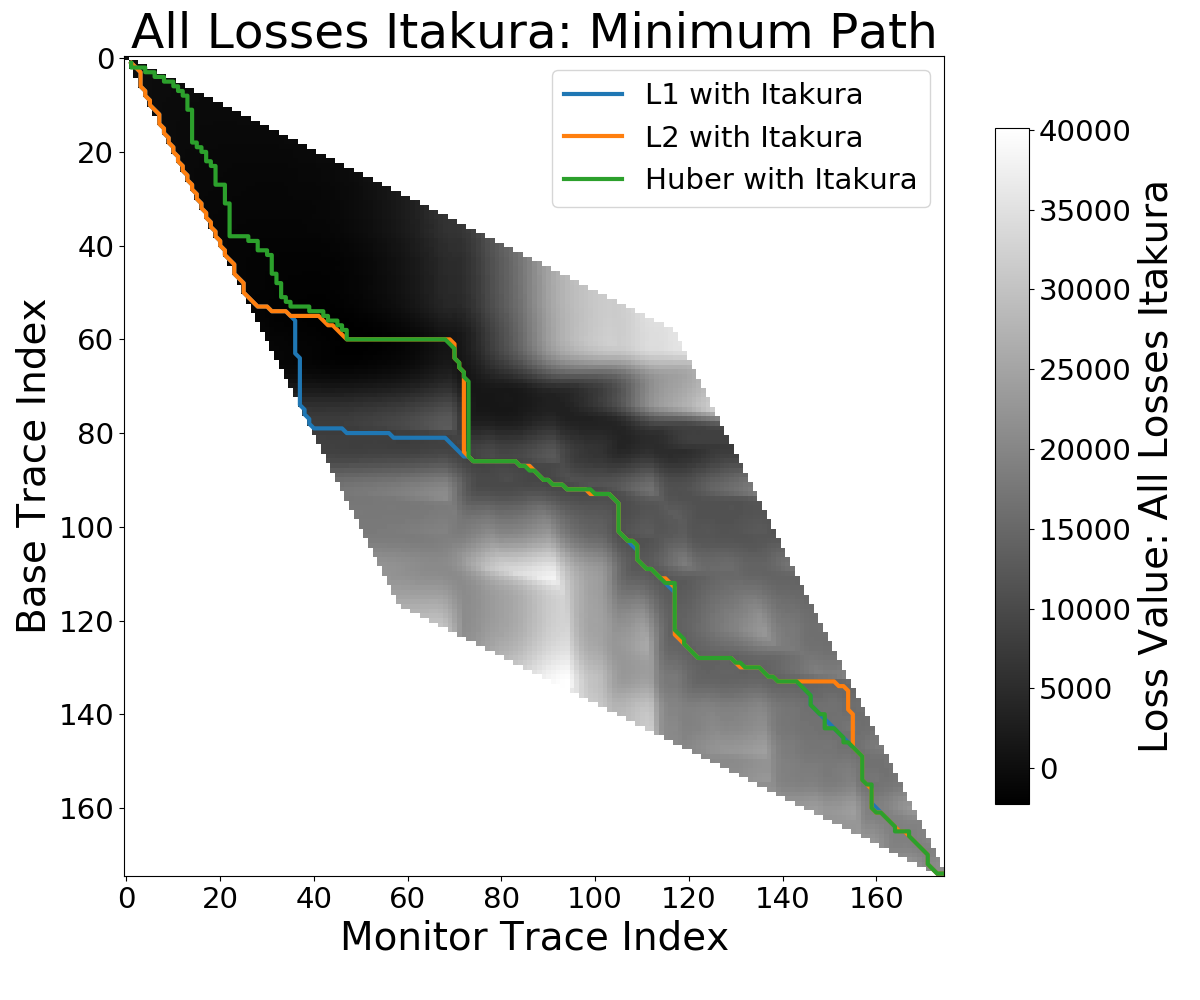
\includegraphics[width=.3\textwidth]{figures/minimum_path_all_losses_itakura_.png} \label{fig:itakura}
    }
    ~
    \subbottom[\citet{Sakoe1978} Disc]{%
     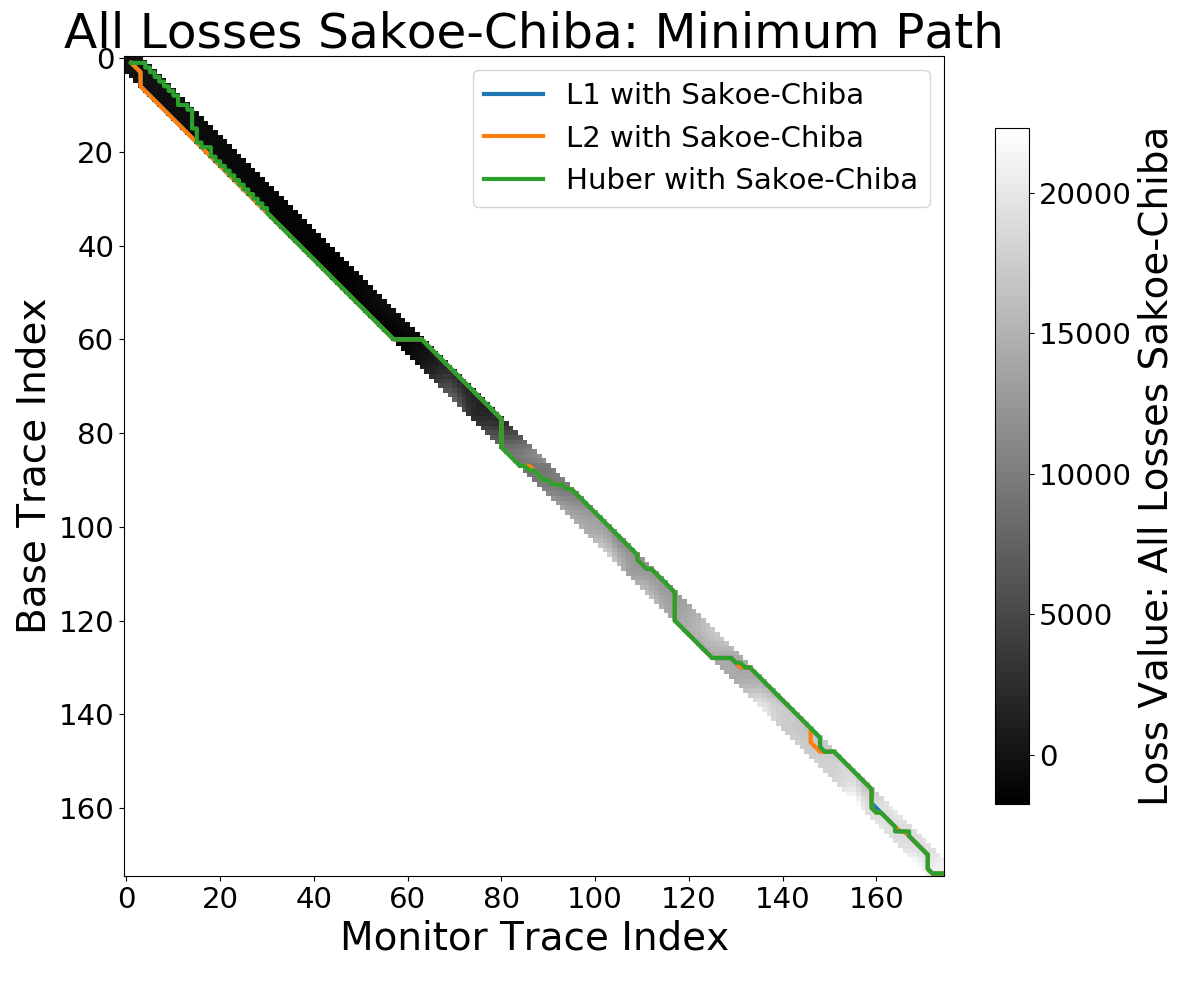
\includegraphics[width=.3\textwidth]{figures/minimum_path_all_losses_sakoe_chiba_.png} \label{fig:sakoe}
    }
    ~
    \subbottom[LB\_Envelope \citep{keogh2005exact}]{%
     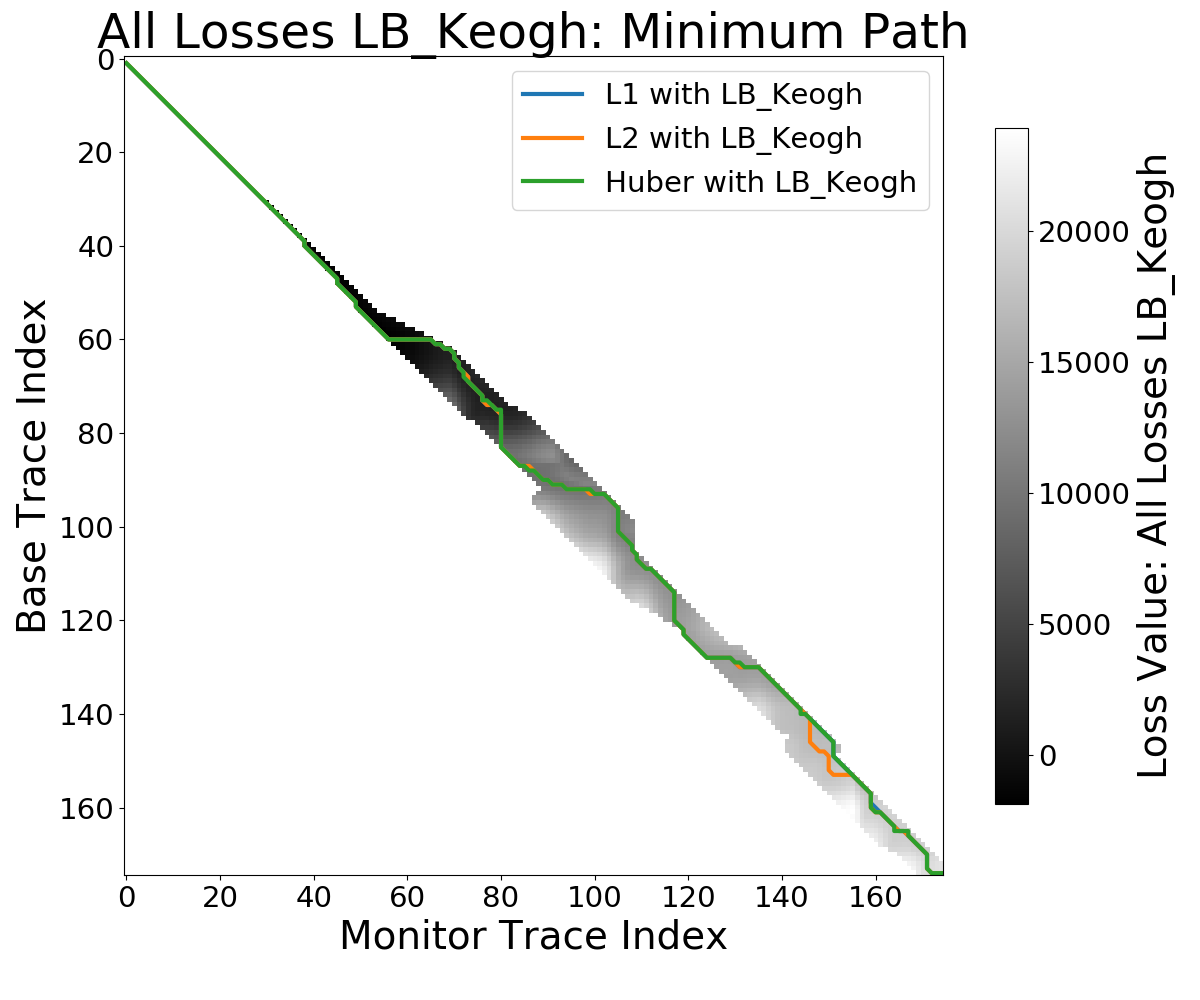
\includegraphics[width=.3\textwidth]{figures/minimum_path_all_losses_lb_keogh_.png}\label{fig:lbk}
    }
\caption{Minimum path for constraint masks for cumulative cost in \ac{dtw}. Images show the optimum path for different loss functions $L_1$, $L_2$, and Huber loss \citep[from][]{dramsch2019dtw}}
\label{fig:constraints}
\end{figure} 
% dramsch2019dtw
\citet{dramsch2019dtw} presents a tutorial of \acf{dtw}. \ac{dtw} is a powerful signal processing tool introduced to 4D seismic analysis by \citep{Hale2013} on synthetic data. 4D seismic data relies on alignment of the seismic volumes. This enables interpreters to compare the amplitudes differences of the data. Due to the capability of \ac{dtw} to match arbitrary time-series, it is applicable to 4D time shifts, seismic-well ties, well-to-well ties, and seismic pre- and post-stack migration \citep{Luo*2014}.  \ac{dtw} is known to be computationally slow and expensive, while extracting poor matches on seismic field data. This tutorial paper goes into detail of the \ac{dtw} algorithm, exploring similarity measures, optimization, and constraints interactively through reproducible implementation in Python.

\begin{algorithm}
\begin{algorithmic}
\Procedure{DTW}{$a,b$}
\State Given: Trace $a$ and Trace $b$ of lengths $n$.
\Function{Calculate distance matrix $D$}{$a,b$}
    \State $D \gets dist(a,b)$
\EndFunction
\Function{Calculate Cumulative Cost $C$}{$D$}
\State $C[0,0] \gets 0$
\For {$i = 1$ to $n$} \Comment{Populate Edge}
    \State $C[0,i] \gets D[0,i] + C[0,i-1]$
    \State $C[i,0] \gets D[i,0] + C[i-1,0]$
\EndFor
\For {$i = 1$ to $n$} \Comment{Fill Cumulative Cost Matrix}
    \For {$j = 1$ to $n$} 
        \State $C_{min} \gets \textbf{min} \{C[i,j-1], C[i-1,j-1], C[i-1,j]\}$
        \State $C[i,j] \gets D[i,j] + C_{min}$
    \EndFor
\EndFor
\EndFunction
\Function{Backtrack minimum cost path $P$}{$C$}
\State $P \gets C[n,n]$
\While {$i > 0 | j > 0$}
    \State $i, j \gets \textbf{index} \{ P[last] \}$
    \State $C_{min} \gets \textbf{min} \{C[i,j-1], C[i-1,j-1], C[i-1,j]\}$
    \State $P.\textbf{append} \gets \textbf{index} \{ C_{min} \}$
\EndWhile
\EndFunction
\State \Return {P}
\EndProcedure
\end{algorithmic}
\caption{\acl{dtw} algorithm consists of calculating the element-wise distance matrix, cumulative cost and then find the optimal path in the cumulative cost matrix} \label{dtw}
\end{algorithm}

The \ac{dtw} algorithm, represented in \cref{dtw}, relies on calculating a distance matrix sample-wise between two traces. This is the first avenue of optimization we explore in this paper. The commonly used $L_1$ norm to calculate the distance norm is shown to perform worst out-of-the-box calculating $|b-a|$. Alternatively, the euclidean distance or $L_2$ norm can be used, which modifies the calculation to $(b-a)^2$. The difference between $L_1$ and $L_2$ is significant in the sense that the $L_1$ norm is not differentiable or convex, however it scales linearly for outliers. The $L_2$ norm converges fast close to zero, however the error "explodes" for outliers. We introduce a constraint used in convex optimization, which combines the advantages of the $L_1$ norm and $L_2$ norm, namely the Huber loss:

\begin{equation}
L_\delta (a, b) = 
\begin{cases}
 \frac{1}{2} (b-a)^2 & \text{for } |b-a| \le \delta, \\
 \delta (|b-a| - \frac{1}{2} \delta), & \text{otherwise.}
\end{cases}
\label{eq:huber}
\end{equation}

which is convex for small values, scales linearly for outliers and is differentiable for all values of $\mathbb{R}$, with $\delta$ being a scaling factor.

Additionally, the search space on the cumulative distance matrix can be constrained to both increase performance and avoid non-optimal solutions. The different contraint strategies are presented in \cref{fig:constraints}. The Itakura parallelogram \citep{Itakura1975} in \cref{fig:itakura} describes a parallelogram that that has the largest width agress the diagonal of the matrix, providing the most flexibility for the \ac{dtw} algorithm in the center parts of the seismic traces. The Sakoe-Chiba disc \citep{Sakoe1978} follows a different strategy, which provides a constant maximum warp path. This strategy in \cref{fig:sakoe} introduces a global maximum time shift. Contrary to these two global constraints, we introduce the LB\_Keogh \citep{keogh2005exact} constraint in the paper. This lower bounding method provides a mathematical lower bound for the \ac{dtw} algorithm. We use this lower bound to constrain the warp path, which provides larger variability to high amplitude areas, where cycle-skipping can occur, presented in \cref{fig:lbk}. The results of combining the Huber loss with the LB\_Keogh constraint are presented in \cref{fig:time-shifts-warped}.

\begin{figure}[!ht]
    \centering
    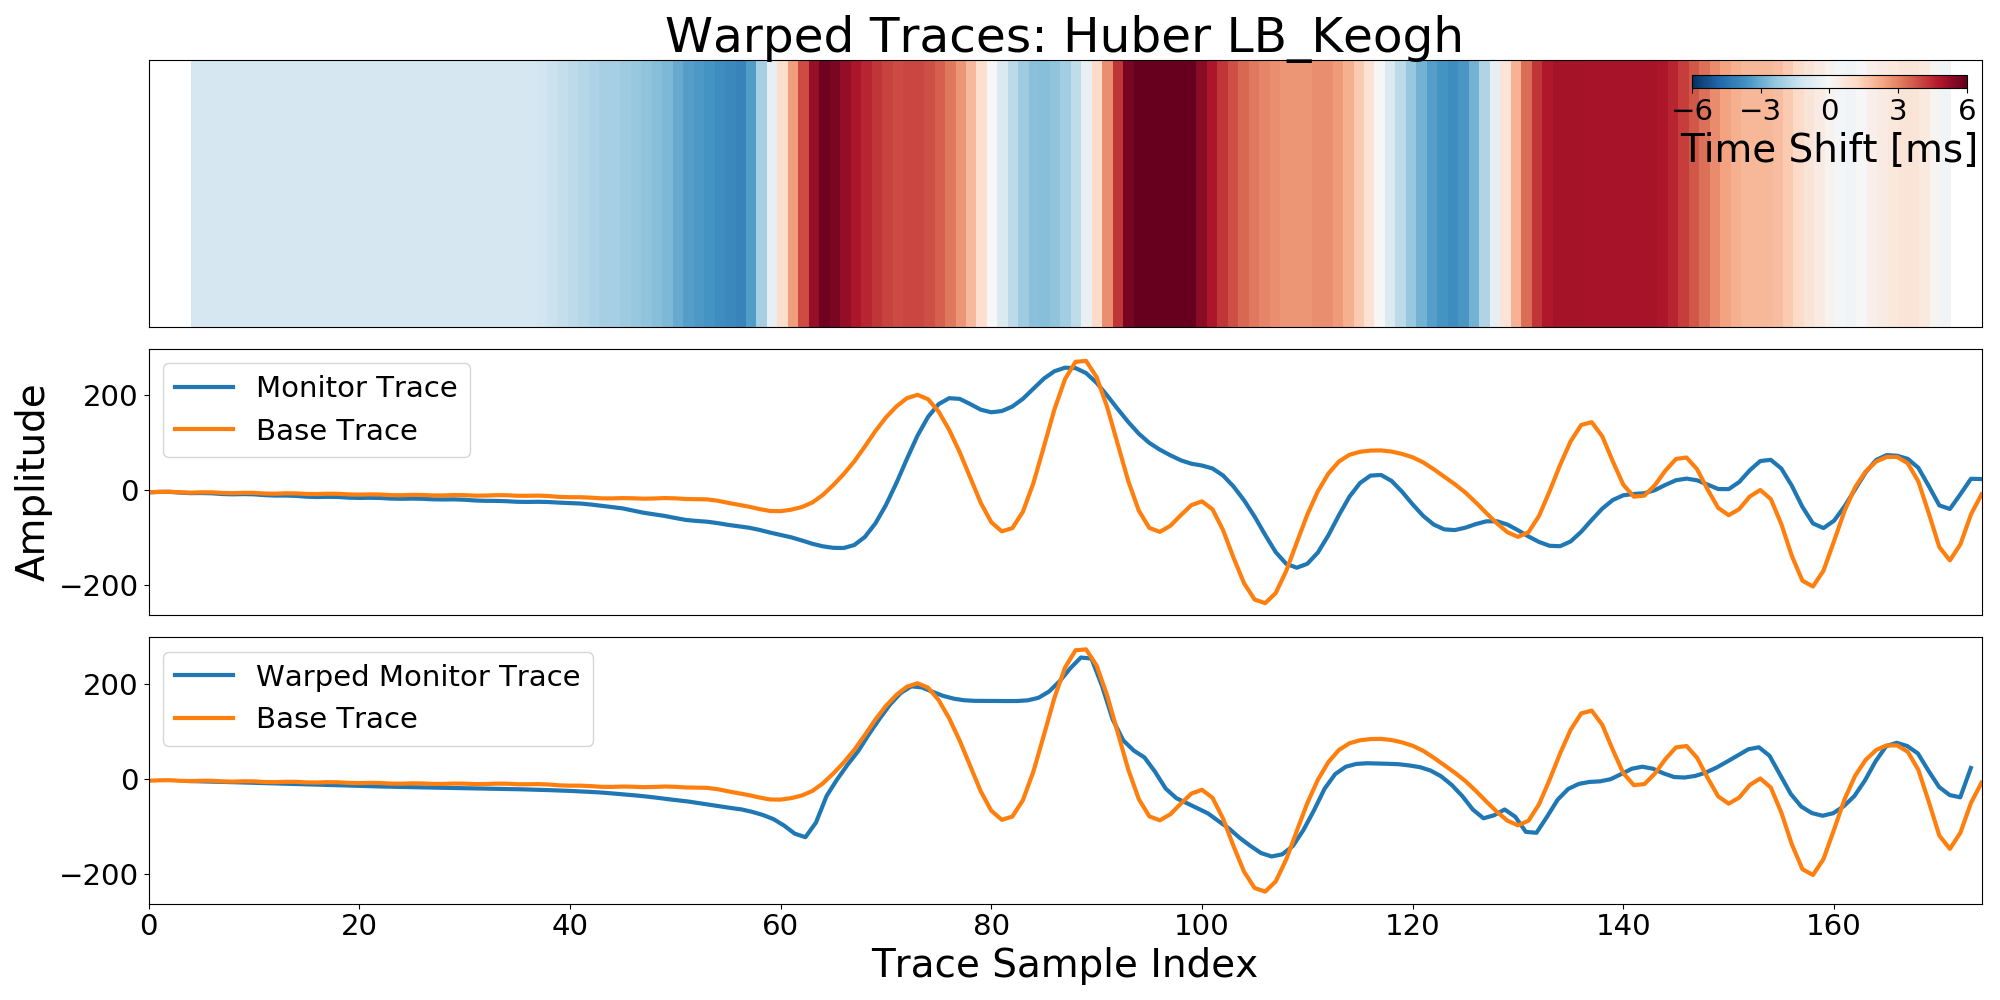
\includegraphics[width=\textwidth]{figures/time_shift_huber_lb_keogh.png}
    \caption{Time shifts and warped traces \citep[from][]{dramsch2019dtw}}
    \label{fig:time-shifts-warped}
\end{figure}

% dramsch2018information
In the workshop paper \citetitle{dramsch2018information} \citep{dramsch2018information} the insight from applying the LB\_Keogh constraint was transferable to \acp{cnn}. \acp{cnn} apply a windowed convolution to the input data. Windowed areas of non-stationary physical data can be offset from the usually baselevel of an amplitude of zero. In the case of seismic data, traces tend to be zero-centered. In the case of a simple activation of a single neuron in a \ac{nn} with $\sigma(w\cdot x + b)$ (cf. \cref{section:nn}), this equates to a bias of $b=0$. Seismic data contains sections that fall within the range of most patches, where the reflection response is entirely offset from zero, which equates to a mean-shift within the network. This paper served as a preliminary study for \citet{dramsch2019complex}, which explores a solution for this property of patch-based training in \acp{cnn} that deteriorates the generalization.

\begin{figure}
    \centering
    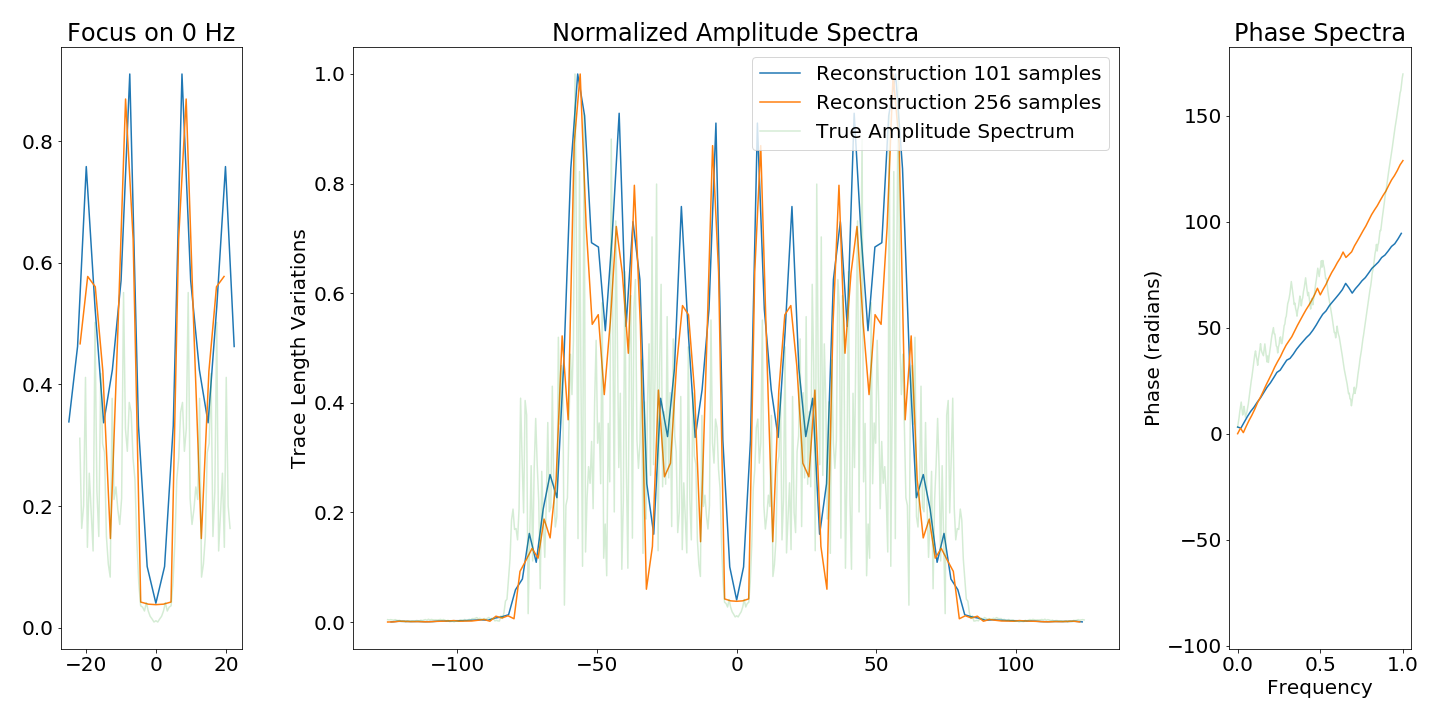
\includegraphics[width=\textwidth]{figures/information-windowing.png}
    \caption{Normalized spectra of windows of trace with "offset" zero. Aliasing of the low frequencies is visible.Phase information not reconstructed from windowed data, slope depending on the window size. Data tapered before \ac{fft} \citep[from][]{dramsch2018information}}
    \label{fig:seismic-window}
\end{figure}

\aclp{nn} apply real-valued transformations on the data, discarding phase information entirely. \cref{fig:seismic-window} shows the spectra of the full trace in green as a background, with two selected cutouts of different sizes overlaid. It is clear that both windows show a sufficiently good reconstruction of the original amplitude spectrum, except for the offset at the low frequencies. The slope of the phase spectrum is reconstructed somewhat by the larger window, but non can reconstruct the notch. Many deterministic signals contain significant information in the phase of the signal. Discarding the phase information leads to low-frequency aliasing analogous to the Nyquist-Shannon theorem for high frequencies.

% dramsch2019complex
In the paper \citetitle{dramsch2019complex} \citep{dramsch2019complex} I explore complex-valued deep convolutional networks to leverage non-linear feature maps and show that in non-stationary data, the phase content improves generalization of \acp{cnn}. Furthermore, complex-valued networks result in a smaller network with better performance compared to a larger real-valued network. In this study I implemented a deep convolutional \acl{ae} to compress 2D slices from a 3D seismic cube to evaluate the reconstruction error. There is a difference of network implementations, where complex-valued neurons are represented as two feature maps, one for the real component and complex component each. Therefore, matching the networks proved to be a complicated task, which led me to build four different architectures that get progressively bigger and compare the results.

The work in \citetitle{dramsch2019complex} \citep{dramsch2019complex} was in part based on reconstruction to test lossy compression and reconstruction of seismic data. Another reason to implement an unsupervised method was the limited availability of realiable interpretations of seismic data. Defining a decision boundary for seismic interpretation is only in the beginning stages of research, which leads us to the decision to inspect reconstructed seismic numerically as signal analysis is well-explored in seismic data processing. Therefore, analysing the result in the \ac{fk}-domain was possible and gave additional insight to the denoising effect of the \ac{ae}.

Nevertheless, some interpretations are available openly and companies often have a plethora of interpretations and re-interpretations of seismic data, making automatic seismic interpretation a topic of interest as evidenced by \cref{tab:geonn}. However, \aclp{dnn} are notorious for needing large numbers of diverse annotated samples. That is often prohibitive to geoscience applications of \acl{ml}. In \citetitle{dramsch2018deep} \citep{dramsch2018deep} we show that \aclp{sota} \aclp{cnn} pre-trained on ImageNet can be transferred to perform \acl{asi}. \cref{fig:asi} shows the results of a fully trained network compared to a pre-trained network. The pre-trained network decreases both training time and data requirements significantly, while not compromising accuracy. A pre-trained network with diverse generalizable learned filters seems to alleviate some limitations of smaller non-diverse data sets used in the fine-tuning process.

\begin{figure}[!ht]
    \subbottom[Waldeland CNN trained from scratch]{%
     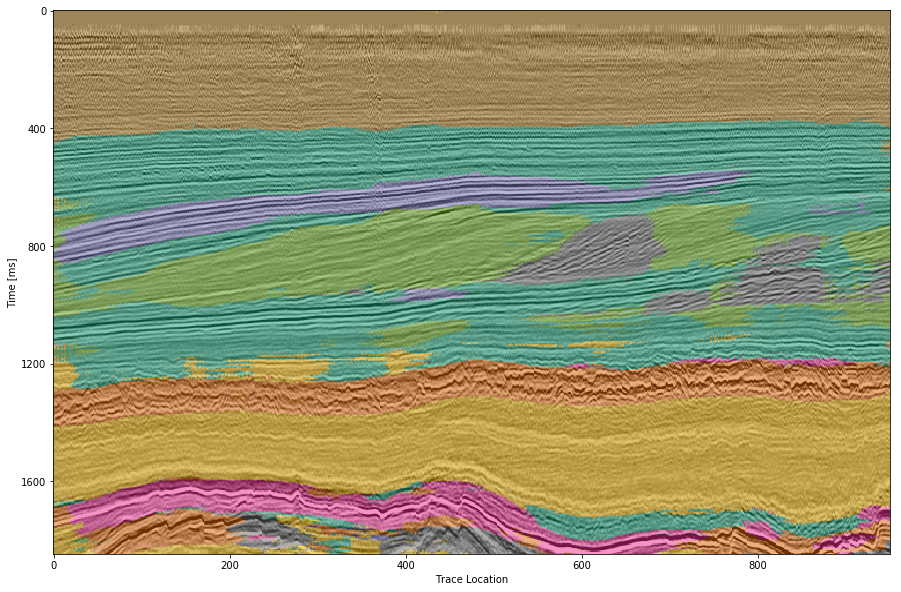
\includegraphics[width=.5\textwidth]{figures/pred1_i.png} \label{fig:asi_pred_waldeland}
    }
    \subbottom[Pre-trained VGG-16]{%
     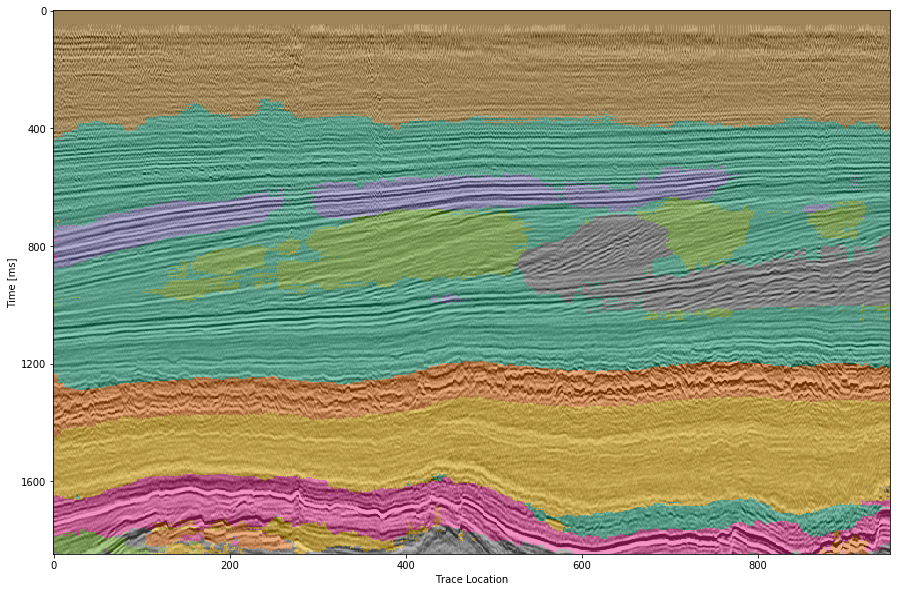
\includegraphics[width=.5\textwidth]{figures/vgg1_i.png} \label{fig:asi_pred_vgg}
    }
\caption{\acl{asi} on two networks, trained from scratch and fine-tuned on pre-trained VGG-16 architecture. The pre-trained network generating a more consistent seismic interpretation, however showing an overall deficiency in diverse training data \citep[from][]{dramsch2018deep}}
\label{fig:asi}
\end{figure}

This chapter summarizes the foundational work conducted to enable the developments of concrete applications of \acl{dl} in geophysics. These foundations touch on signal processing fundamentals in 4D seismic exploring metrics and constraints, then introducing a new constraint for \acl{dtw} in 4D seismics. The work in \aclp{dnn} includes an investigation into aliasing of patch-based training of \aclp{cnn} and including phase information in complex-valued neural networks. Finally, leading to an exploration of transfer learning for efficient training of deep learning models in \acl{asi}.